\documentclass[tikz,crop]{standalone}
\usepackage{amsmath}
\usepackage{amssymb}
\usepackage[english]{babel}
\usepackage[utf8]{inputenc}
\usepackage[T1]{fontenc}
\usepackage{euler}

\usepackage{tikz,pgfplots}
\usetikzlibrary{matrix, shapes, arrows, positioning}

\begin{document}

	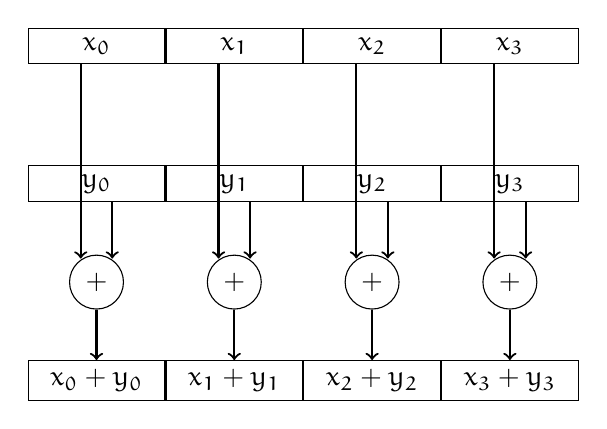
\begin{tikzpicture}[node distance=1.75cm]
		
		\node[rectangle,draw,text width=1.5cm,align=center,] (X0) {$x_0$};
		\node[rectangle,draw,text width=1.5cm,align=center, right of=X0] (X1) {$x_1$};
		\node[rectangle,draw,text width=1.5cm,align=center, right of=X1] (X2) {$x_2$};
		\node[rectangle,draw,text width=1.5cm,align=center, right of=X2] (X3) {$x_3$};
		
		\node[rectangle,draw,text width=1.5cm,align=center,below of=X0] (Y0) {$y_0$};
		\node[rectangle,draw,text width=1.5cm,align=center,below of=X1] (Y1) {$y_1$};
		\node[rectangle,draw,text width=1.5cm,align=center,below of=X2] (Y2) {$y_2$};
		\node[rectangle,draw,text width=1.5cm,align=center,below of=X3] (Y3) {$y_3$};
		
		\node[circle,draw,align=center,yshift=0.5cm,below of=Y0] (+0) {$+$};
		\node[circle,draw,align=center,yshift=0.5cm,below of=Y1] (+1) {$+$};
		\node[circle,draw,align=center,yshift=0.5cm,below of=Y2] (+2) {$+$};
		\node[circle,draw,align=center,yshift=0.5cm,below of=Y3] (+3) {$+$};
		
		\node[rectangle,draw,text width=1.5cm,yshift=0.5cm,align=center,below of=+0] (E0) {$x_0 + y_0$};
		\node[rectangle,draw,text width=1.5cm,yshift=0.5cm,align=center,below of=+1] (E1) {$x_1 + y_1$};
		\node[rectangle,draw,text width=1.5cm,yshift=0.5cm,align=center,below of=+2] (E2) {$x_2 + y_2$};
		\node[rectangle,draw,text width=1.5cm,yshift=0.5cm,align=center,below of=+3] (E3) {$x_3 + y_3$};
		
		\draw[thick,->] ([xshift=-0.2cm]X0.south) -- ([xshift=-0.2cm,yshift=-0.05cm]+0.north);
		\draw[thick,->] ([xshift=+0.2cm]Y0.south) -- ([xshift=+0.2cm,yshift=-0.05cm]+0.north);
		
		\draw[thick,->] ([xshift=-0.2cm]X1.south) -- ([xshift=-0.2cm,yshift=-0.05cm]+1.north);
		\draw[thick,->] ([xshift=+0.2cm]Y1.south) -- ([xshift=+0.2cm,yshift=-0.05cm]+1.north);
		
		\draw[thick,->] ([xshift=-0.2cm]X2.south) -- ([xshift=-0.2cm,yshift=-0.05cm]+2.north);
		\draw[thick,->] ([xshift=+0.2cm]Y2.south) -- ([xshift=+0.2cm,yshift=-0.05cm]+2.north);
		
		\draw[thick,->] ([xshift=-0.2cm]X3.south) -- ([xshift=-0.2cm,yshift=-0.05cm]+3.north);
		\draw[thick,->] ([xshift=+0.2cm]Y3.south) -- ([xshift=+0.2cm,yshift=-0.05cm]+3.north);
		
		\draw[thick,->] (+0) -- (E0);
		\draw[thick,->] (+1) -- (E1);
		\draw[thick,->] (+2) -- (E2);
		\draw[thick,->] (+3) -- (E3);

		


	\end{tikzpicture}
		
\end{document}
	